\subsection{Testaufbau}
Im Folgenden wird die Arbeitsumgebung, d.h. Entwicklungsplattform, sowie Hard- 
und Software-Komponenten erläutert.

Als Betriebsystem wird Windows 7 32 und 64 Bit verwendet.
 
Es liegen folgende Hardware-Komponenten vor:
\begin{itemize}
\item AX-12A
\item OpenCM 485 Expansion Board
\item OpenCM9.04-C
\end{itemize}

Es liegen folgende Software-Komponenten vor:
\begin{itemize}
\item ROBOTIS\_OpenCM
\item Visual Studio 2013 Community
\end{itemize}

% ------------------------------
\begin{table}[H]
\caption{Investitionskosten}\label{tab:Investitionskosten}
\renewcommand{\arraystretch}{1.5} 
\newcolumntype{C}[1]{>{\centering\arraybackslash}p{#1}}
\centering
\begin{tabular}{|p{5cm}|p{1.5cm}|p{5cm}|p{1.5cm}|}
\hline 
\textbf{Hardware} & \textbf{Kosten} & \textbf{Software} & \textbf{Kosten} \\ 
\hline 
AX-12A & \EUR{46,80} & ROBOTIS\_OpenCM &  \\ 
\hline 
OpenCM 485 Expansion Board & \EUR{27,50} & Visual Studio 2013 Community & \\ 
\hline 
OpenCM9.04-C & \EUR{21,50} &  &   \\ 
\hline
\multicolumn{4}{|l|}{} \\ 
\hline
\textbf{Versandkosten} & \EUR{11,29} & & \\ 
\hline
\textbf{Summe} & \textbf{\EUR{107,09}} & & \\ 
\hline 
\end{tabular} 
\end{table}

\begin{figure}[H]
	\centering
	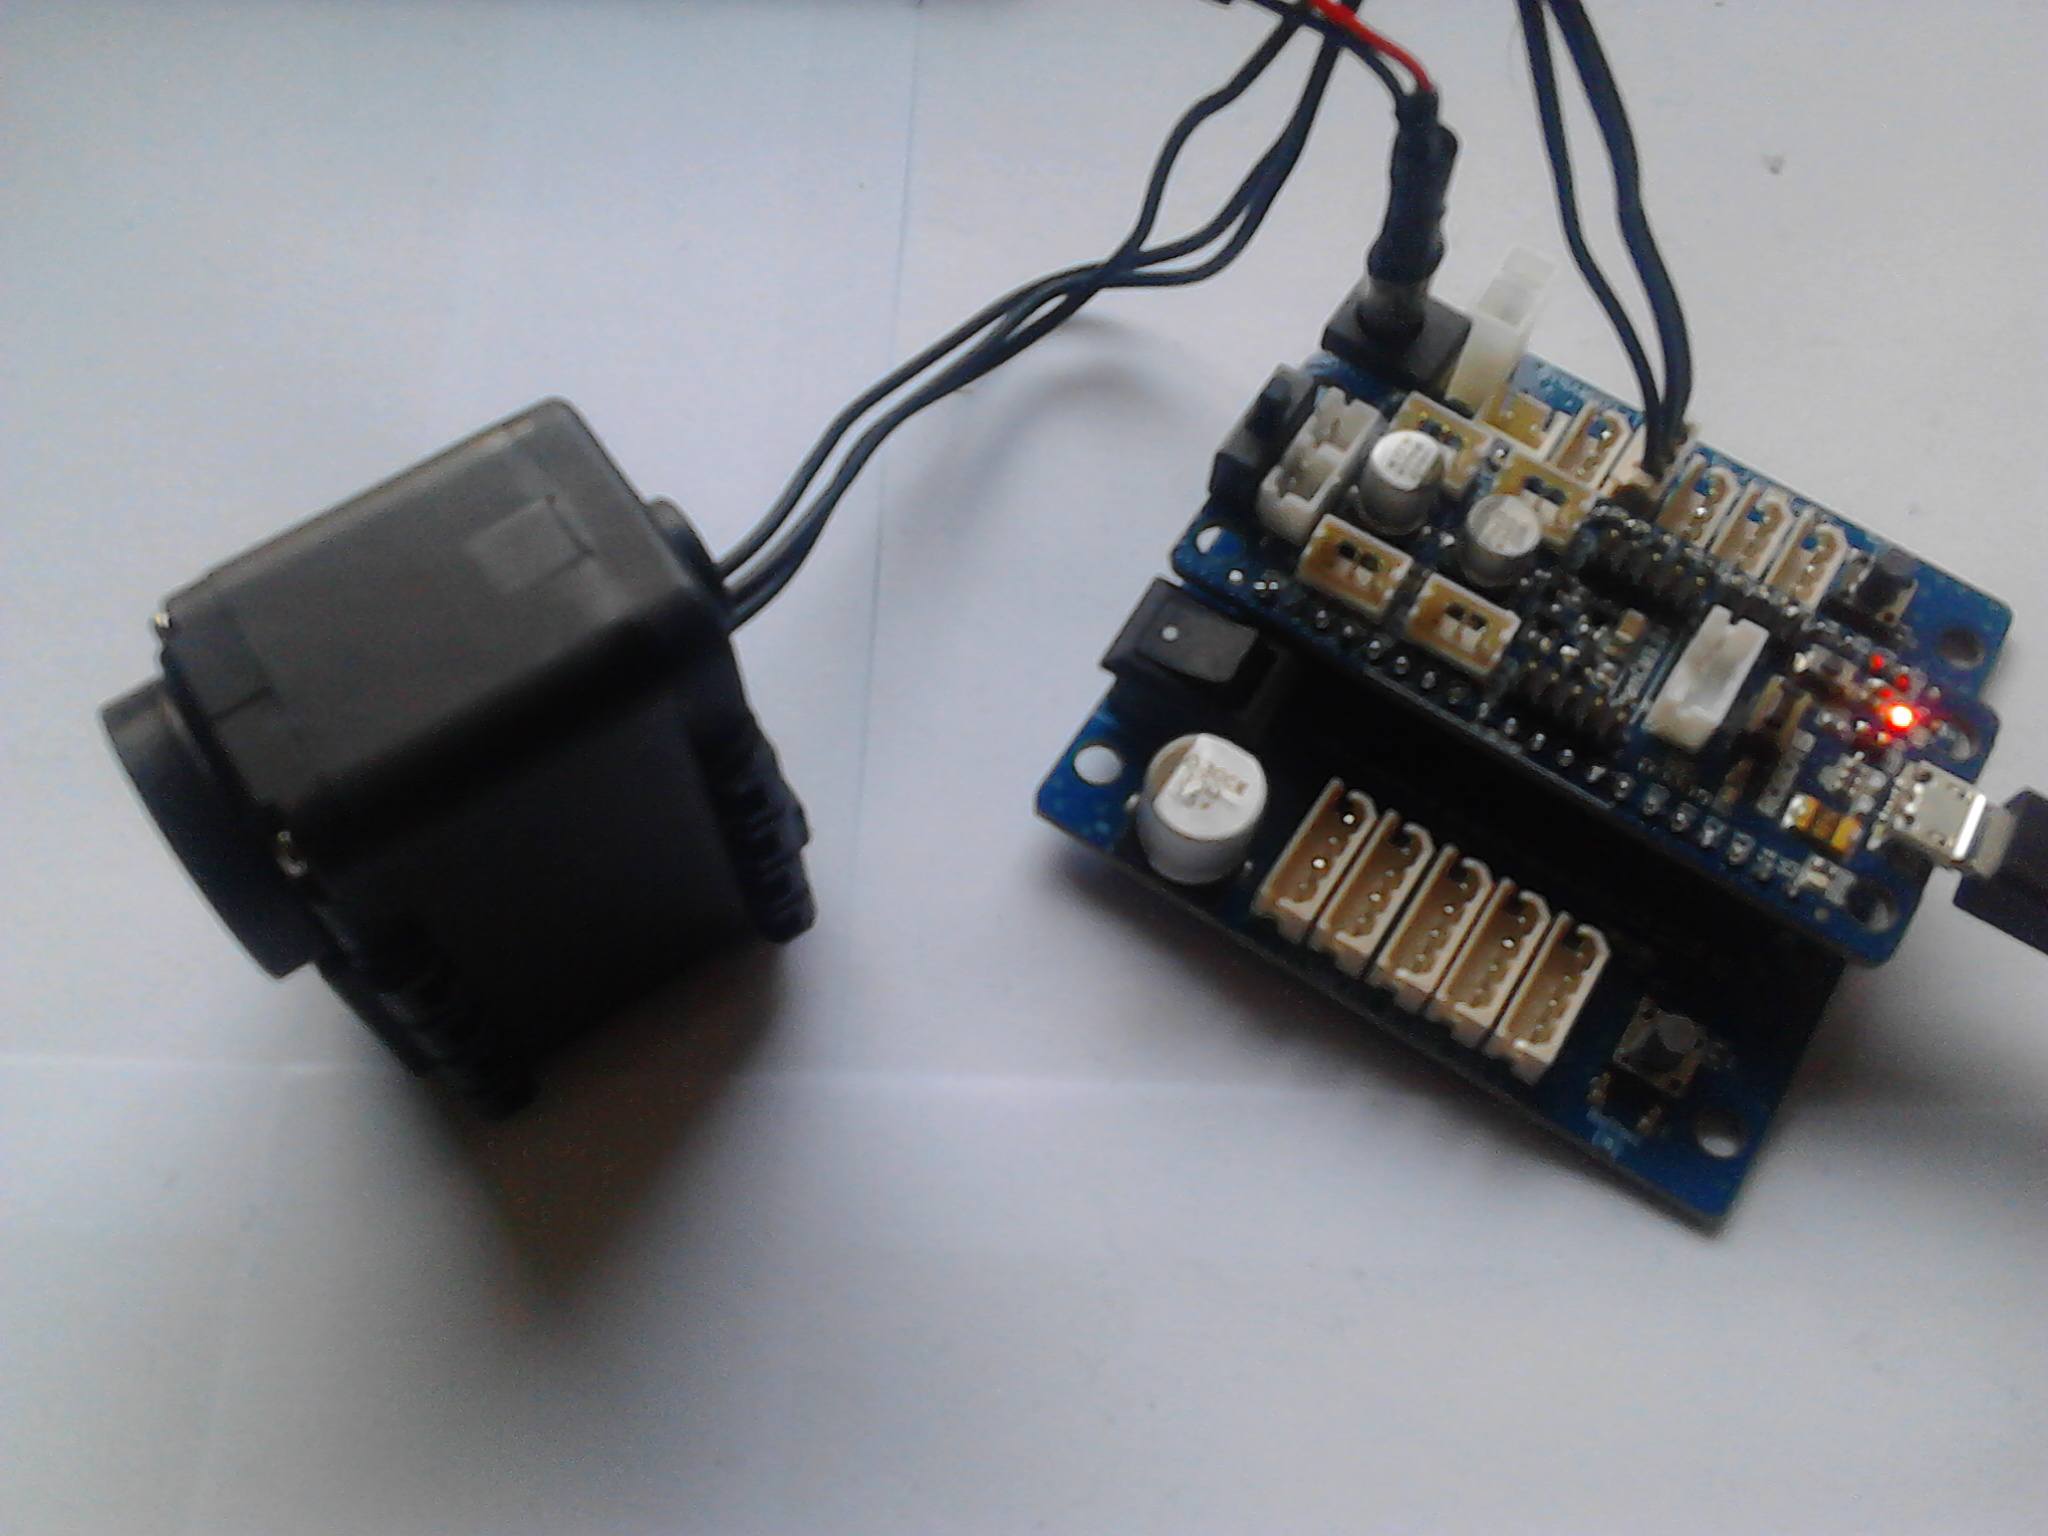
\includegraphics[width=0.85\textwidth]{03_Grafiken/Grundlagen/Testaufbau/Komponenten.jpg}
	\caption[Testaufbau]{Testaufbau}
	\label{fig:Testaufbau}
\end{figure}


